%- HandOut Flag -----------------------------------------------------------------------------------------
\newif\ifHandout

%- D0cum3nt ----------------------------------------------------------------------------------------------
\documentclass[beamer,10pt]{standalone}   
%\documentclass[beamer,10pt,handout]{standalone}  \Handouttrue  

%- HandOut Flag -----------------------------------------------------------------------------------------
\ifHandout
	\setbeameroption{show notes} %print notes   
\fi

	
%- Packages ----------------------------------------------------------------------------------------------
\usepackage{custom-style}
\usetikzlibrary{positioning}
\usepackage{multicol}


%--Beamer Style-----------------------------------------------------------------------------------------------
\usetheme{toninus}
\usepackage{animate}
\usetikzlibrary{positioning, arrows}
\usetikzlibrary{shapes}
\usepackage{ifthen}

\begin{document}
%-------------------------------------------------------------------------------------------------------------------------------------------------
\begin{frame}{From \emph{configurations} to \emph{states}}
\begin{columns}[T]
	\begin{column}{0.5\textwidth}
		\begin{center}
			\resizebox{\textwidth}{!}{		
				\pgfmathtruncatemacro\steps{50}
				\pgfmathtruncatemacro\maxtheta{30}
				\pgfmathtruncatemacro\pi{3.14}
				\begin{animateinline}[autoplay,loop]{10} % 5 fps, same as 0.2 s transduration
				  \multiframe{\steps}{i=0+1}{
				    \begin{tikzpicture}
				    \pgfmathsetmacro\fraction{\i/(\steps-1)}
					\pgfmathsetmacro\theta{\maxtheta*cos(360*\fraction)-90}
					\pgfmathsetmacro\v{-1*sin(360*\fraction)}
				
				    %frame
				    \draw[draw=none] (-6,-8) rectangle (6,6);		
					% Support
					\coordinate (o) at (0,0);
					\node[cross out,draw,black!10] (0,0){};
					\node[circle,draw,black!10] (0,0){};
					% Bob's trajectory
					\draw[blue,line width=1mm] (0,0) circle (4);
					% Rod + Bob
					\draw[dashed] (0,0) -- (\theta:4) node[fill,circle,red](m){};

					% Velocity
					\ifthenelse{\equal{\i}{0}}
           			{}
           			{\draw[-latex,green!80!black,line width=1mm] (m) -- node[green!80!black,below right]{$\vec{v}$}($(m)!\v!-90:(o)$);}
				    \end{tikzpicture}
				  }
				\end{animateinline}
			}
		\end{center}
	\end{column}
	\begin{column}{0.5\textwidth}
		\begin{itemize}
			\item Knowing the position is not sufficient to determine the evolution of the system.
			\item (Displacement encode statics, one must know how configurations evolves in time)
			\item One needs to know also the velocity (or better, the momentum).
		\end{itemize}

		\vspace{1em}
		\onslide<2->{
			\begin{upshotblocksimp}
				Upshot:
				Configurations $\neq$ \emph{States}
			\end{upshotblocksimp}			
		}
	\end{column}
\end{columns}
\end{frame}
\note[itemize]{
	\item
}
%-------------------------------------------------------------------------------------------------------------------------------------------------

%-------------------------------------------------------------------------------------------------------------------------------------------------
\begin{frame}{Quick reminder: Trajectories, velocities, Tangent spaces}



	\begin{columns}
			\begin{column}{.6\linewidth}
				\only<1>{\includegraphics[width=\textwidth]{Pictures/Vector1} }
				\only<2>{\includegraphics[width=\textwidth]{Pictures/Vector2} }
				\only<3->{\includegraphics[width=\textwidth]{Pictures/Vector3} }
			\end{column}
			\begin{column}{.4\linewidth}
				\begin{itemize}
					\item Well defined notion of smooth curves $C^\infty(\mathbb{R},M)$ on smooth manifolds.
					\item<2-> Velocity of curves can be computed through charts.
				\end{itemize}
			\end{column}				
	\end{columns}
		\vfill
		\begin{itemize}
			\item<3-> Comparing velocities in local chars yields an equivalence relations of curves passing through a point $p \in M$
		\end{itemize}
		
		\vfill
		\onslide<4->{
		\begin{defblock}[Tangent space at $p\in M$]
			\begin{displaymath}
				T_p M \coloneqq
   				\left\{
				\parbox{.55\linewidth}{Vector space of equivalence classes of curves \\with equal local velocity at $p\in M$.}
				 \right\}.
			\end{displaymath}
		\end{defblock}
		}
\end{frame}
\note[itemize]{
	\item
}
%-------------------------------------------------------------------------------------------------------------------------------------------------

%-------------------------------------------------------------------------------------------------------------------------------------------------
\begin{frame}{Phase Space (I)}
\begin{columns}[T]
	\begin{column}{0.5\textwidth}
		\begin{center}
			\resizebox{\textwidth}{!}{
				\begin{tikzpicture}
					\node[draw=none] (o) at (0, 0) {o};
				    %frame
				    \draw[draw=none] (-6,-8) rectangle (6,6);				
					\draw[draw=none](0,0)--(-90:4)node[circle, fill, minimum size=5pt,
				              inner sep=0pt, outer sep=0pt](p){};
					\draw[green,line width=1mm] ($ (p)!3.5cm!90:(o) $) -- ($ (p)!3.5cm!270:(o) $);
					\draw[green,dashed,line width=1mm] ($ (p)!4.5cm!90:(o) $) -- ($ (p)!4.5cm!270:(o) $);
					\draw[blue,line width=1mm] (0,0) circle (4);
				\end{tikzpicture}
			}
			%
		\end{center}
	\end{column}
	\begin{column}{0.5\textwidth}
 		\begin{itemize}
 			\item consider {\bf a} configuration.
 			\item all possible velocities are encoded by points on the tangent line at the given configuration \\(\emph{Tangent space}).
 		\end{itemize}
	\end{column}
\end{columns}
\end{frame}
\note[itemize]{
	\item
}
%-------------------------------------------------------------------------------------------------------------------------------------------------



%-------------------------------------------------------------------------------------------------------------------------------------------------
\begin{frame}{Phase Space (II)}
\begin{columns}[T]
	\begin{column}{0.5\textwidth}
		\begin{center}
			\only<1>{
			\resizebox{\textwidth}{!}{
				\begin{tikzpicture}
					\node[draw=none] (o) at (0, 0) {o};
				    %frame
				    \draw[draw=none] (-6,-8) rectangle (6,6);						
					\foreach \x in {0,30,...,360}{
						\draw[draw=none](0,0)--(\x:4)node[circle, fill, minimum size=5pt,
					              inner sep=0pt, outer sep=0pt](p){};
					\draw[green,line width=1mm] ($ (p)!3.5cm!90:(o) $) -- ($ (p)!3.5cm!270:(o) $);
					\draw[green,dashed,line width=1mm] ($ (p)!4.5cm!90:(o) $) -- ($ (p)!4.5cm!270:(o) $);
					}
						\draw[blue,line width=1mm] (0,0) circle (4);
				\end{tikzpicture}
			}}
			%
			\only<2->{
			\resizebox{.7\textwidth}{!}{
				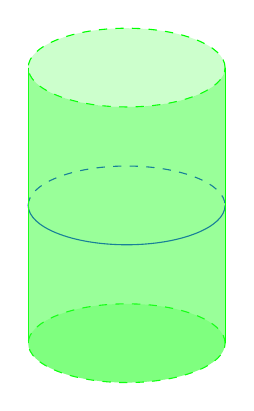
\begin{tikzpicture}
					\draw[green,dashed,fill=green!20] (0,0) ellipse (1.25 and 0.5);
					\draw [blue](-1.25,-1.75) arc (180:360:1.25 and 0.5);
					%\draw [blue,dashed] (-1.25,-3.5) arc (180:360:1.25 and -0.5);
					\draw[green,dashed,fill=green!20] (0,-3.5) ellipse (1.25 and 0.5);
					\draw [blue,dashed] (-1.25,-1.75) arc (180:360:1.25 and -0.5);
					\draw [green](-1.25,0) -- (-1.25,-3.5);
					\draw [green](1.25,-3.5) -- (1.25,0);  
					\fill [green!80,opacity=0.5] (-1.25,0) -- (-1.25,-3.5) arc (180:360:1.25 and 0.5) -- (1.25,0) arc (0:180:1.25 and -0.5);
				\end{tikzpicture}		
%				\begin{tikzpicture}
%				  \node[cylinder,draw=black,thick,aspect=0.7,minimum height=4cm,minimum width=2.5cm,shape border rotate=90,cylinder uses custom fill, cylinder body fill=green!30,cylinder end fill=green!10] (A) {\phantom{A}};
%				  \draw[dashed]
%				    let \p1 = ($ (A.after bottom) - (A.before bottom) $),
%				        \n1 = {0.5*veclen(\x1,\y1)-\pgflinewidth},
%				        \p2 = ($ (A.bottom) - (A.after bottom)!.5!(A.before bottom) $),
%				        \n2 = {veclen(\x2,\y2)-\pgflinewidth}
%				  in
%				    ([xshift=-\pgflinewidth] A.before bottom) arc [start angle=0, end angle=180,
%				    x radius=\n1, y radius=\n2];
%				\end{tikzpicture}	
}
			}
		\end{center}
	\end{column}
	\begin{column}{0.5\textwidth}
		\vspace{1.5em}
 		\begin{itemize}
 			\item Consider {\bf all possible} configurations.
 			\item Collect all possible pairs of position/momentum.
 			%\item points on the \emph{Tangent space}
 		\end{itemize}
		\vspace{1.5em} 		
 		\begin{itemize}
 			\item<2-> joining together all "tangent" space in a smooth and non-overlapping manner...
 		\end{itemize}
		\onslide<3->{
			\begin{upshotblocksimp}
				Upshot:
				\color{black}
					Collectively, all the possible tangent vector constitute another manifold called the \emph{Tangent Bundle}
					\begin{displaymath}
						TQ = \coprod_{q \in Q} T_q Q
						~.
					\end{displaymath}
				(\emph{Space of generalized velocities})		
			\end{upshotblocksimp}					
		} 		
	\end{column}
\end{columns}
\end{frame}
\note[itemize]{
	\item  		
 		Collect all possible pair of position and momentum
 		
 		Informally, the tangent bundle of a manifold (which in this case is a circle) is obtained by considering all the tangent spaces (top), and joining them together in a smooth and non-overlapping manner (bottom).

}
%-------------------------------------------------------------------------------------------------------------------------------------------------

%-------------------------------------------------------------------------------------------------------------------------------------------------
\begin{frame}{Phase Space}
\begin{columns}[T]
	\begin{column}{0.5\textwidth}
		\begin{center}
			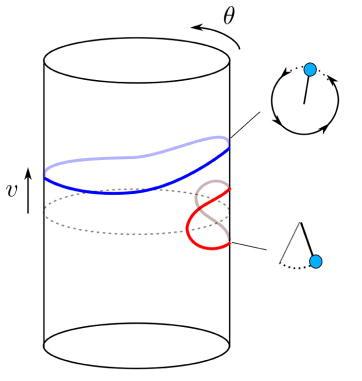
\includegraphics[width=\textwidth]{Pictures/pendo-phasespace}
		\end{center}
	\end{column}
	\begin{column}{0.5\textwidth}
 		\begin{itemize}
 			\item Consider {\bf all possible} configurations.
 			\item Collect all possible pairs of position/momentum.
 		\end{itemize}
		
		\vspace{1em}		
		\begin{defblock}[Phase Space]
			\begin{itemize}
				\item[=] collection of all \emph{states}
				\item[=] set of every possible "initial datas" (sufficient to reconstruct the motion).
			\end{itemize}
		\end{defblock}

		\vspace{1em}				
		\begin{mathblock}
			The Phase space is a \underline{symplectic} smooth manifold $(M)$.
		\end{mathblock}		
		
	\end{column}
\end{columns}
\end{frame}
\note[itemize]{
	\item You get an infinite cylinder (in the case of bipendulum I cannot picture it because we go directly into more than 2 dimensions.
	\item ho disegnato due traiettori sul fase space per mostrare come due natural motions si possono rappresentare bene qui sopra.
	\item per capire il significato di dell'aggettivo simplettico dobbiamo introdurre qualche altro interprete.

}
%-------------------------------------------------------------------------------------------------------------------------------------------------

%-------------------------------------------------------------------------------------------------------------------------------------------------
\begin{frame}{A little clarification on velocities vs momenta}
	\begin{itemize}
		\item In most cases: fixing configuration and velocity fix the state of the system.
		\item However, we consider the dual bundle $T^\ast Q$ as the phase space of the system.
	\end{itemize}
	\pause
	\vfill
	Reasoning: (understand elements in $T^\ast_q Q$ as \emph{mechanical momenta})
	\begin{itemize}
		\item $v\in T_q Q$ measures the rate of change of the displacement $q$ of the system.
		\item $p \in T^\ast_q Q$ measures the rate of change of the kinetic energy of the system w.r.t. a certain variation $\delta v$ of the velocity
		\vspace{-.5em}
		  \begin{alignat*}{2}
			  p: T_q Q &\longrightarrow& \mathbb{R} \\
		  	\delta v &\longmapsto& \delta T
		  \end{alignat*}		
	\end{itemize}

	\pause
	\begin{exblock}[Point-particle in $2D$ space \qquad {\small ( $Q=\mathbb{R}^2$)}]
		\begin{columns}[T]
			\begin{column}{.25\linewidth}
				\resizebox{\textwidth}{!}{
					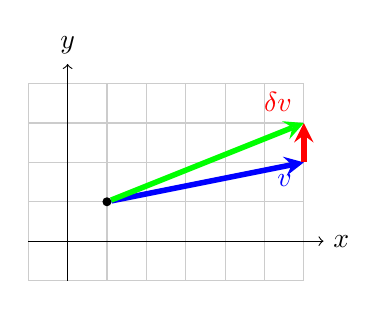
\begin{tikzpicture}
					  \draw[step=.5,thin,gray!40] (-.5,-.5) grid (3,2);
					  \draw[->] (-.5,0)--(3.25,0) node[right]{$x$};
					  \draw[->] (0,-.5)--(0,2.25) node[above]{$y$};
					  \node[draw,circle,fill,inner sep=1pt,] at (.5,.5) (q) {};
					  \draw[line width=2pt,blue,-stealth](q)--(3,1) node[anchor=north east]{$\boldsymbol{v}$};
					  \draw[line width=2pt,red,-stealth](3,1)--(3,1.5) node[anchor=south east]{$\boldsymbol{\delta v}$};
					  \draw[line width=2pt,green,-stealth](q)--(3,1.5) node[anchor=south west]{};
					\end{tikzpicture}
				}			
			\end{column}
			\begin{column}{.80\linewidth}
				Recall from bachelor courses: \quad $
					T = \dfrac{1}{2} m \boldsymbol{v}\cdot \boldsymbol{v} $
				
				Add a perturbation $\boldsymbol \delta v$ to the velocity $\boldsymbol v $.
				{\tiny (Neglecting II-order variations)} :
				\vspace{-.5em}				
				$$ \delta T = m~ \boldsymbol{v}\cdot \boldsymbol{\delta v} = p ( \boldsymbol{\delta v})$$
			\end{column}		
		\end{columns}
	\end{exblock}
	\vfill
	\pause
		\begin{upshotblocksimp}
			Motivation (a posteriori): 
			\color{blue}
			$T^\ast Q$ is naturally symplectic.
		\end{upshotblocksimp}	

\end{frame}
\note[itemize]{
	\item In most cases: fixing configuration adn velocity fix the state of the system.It is customary to consider the dual bundle $T^\ast Q$ as the phase space of the system.
	\item Although fixing a point in $TQ$ fixes the state of the system. In the context of geo. mech. is customary to  understand $T^\ast Q$ as the phase space of the system.
	\item idea: elements of $T_q Q$ measure the rate of change in the displacement of the system, elements of $T_q^\ast Q$ measure the change in kinetic energy of the system (encompassing somewhat the energy encoded by the motion and the system inertia).
	\item Formally, generalized momenta are $P: T_q Q \to \mathbb{R}$ such that, given a state of configuration $q$ and momenta $p$, for any variation $\delta \vec{v}\in T_q Q$, $P(\delta \vec{v})$ measure the variation $\delta T$ in the kinetic energy of the system.
	\item Per completezza: questa caratterizzazione del momento meccanico ha origine dal formalismo Lagrangiano.	
	
	\item What about the definition of linear momentum $\boldsymbol{p} = m \boldsymbol{v}$ learnt in high-school?
				\\
				It's still good since $p = m \boldsymbol{p} \cdot - $ but a little misleading because  based on the existence of an inner product on $Q=\mathbb{R}^3$ which does not exists in general.	
	\item a more precise justification for the fact that "momenta are covector" follows from  the Lagrangian formalism\url{https://math.stackexchange.com/questions/1235015/momentum-a-cotangent-vector}.
}
%-------------------------------------------------------------------------------------------------------------------------------------------------



\end{document}